\documentclass[]{beamer}
% Class options include: notes, notesonly, handout, trans,
%                        hidesubsections, shadesubsections,
%                        inrow, blue, red, grey, brown

% Defines UTF-8 to allow for accents
\usepackage[utf8x]{inputenc}

% Tikz for drawing
\usepackage{tikz}
\usetikzlibrary{arrows}
\usepackage{pgfplots}
\pgfplotsset{compat=newest}
\usepgfplotslibrary{clickable}

% subfigure packages
%\usepackage{caption}
\usepackage{subcaption}
\captionsetup{compatibility=false}
\usepackage{sidecap}

% Smilleys
\usepackage{wasysym}

% Slash over a word
\usepackage{cancel}

% Theme for beamer presentation.
\usepackage{beamerthemesplit} 
% Other themes include: beamerthemebars, beamerthemelined, 
%                       beamerthemetree, beamerthemetreebars  

\title{Controlador AR.Drone} 
\author{André Harder, Jean-Luc Coelho}
\institute{Departamento de Ciência da Computação, UFMG}
% \date{\today}                    % Enter the date or \today between curly braces
\date{}                    % Enter the date or \today between curly braces

\renewcommand{\figurename}{Figura}
\renewcommand{\tablename}{Tabela}

\begin{document}

% Creates title page of slide show using above information
\begin{frame}
  \titlepage
\end{frame}

\section{Controlador AR.Drone}
\subsection{Introdução}

\begin{frame}
\frametitle{Introdução}

O \emph{Parrot AR.Drone} (2.0) é um drone comercial:
\begin{itemize}
\item Quadricóptero com controle individual
\item Câmeras para a frente e para baixo
\item Controlável por \emph{WiFi}
\end{itemize}

\begin{figure}
	\centering
	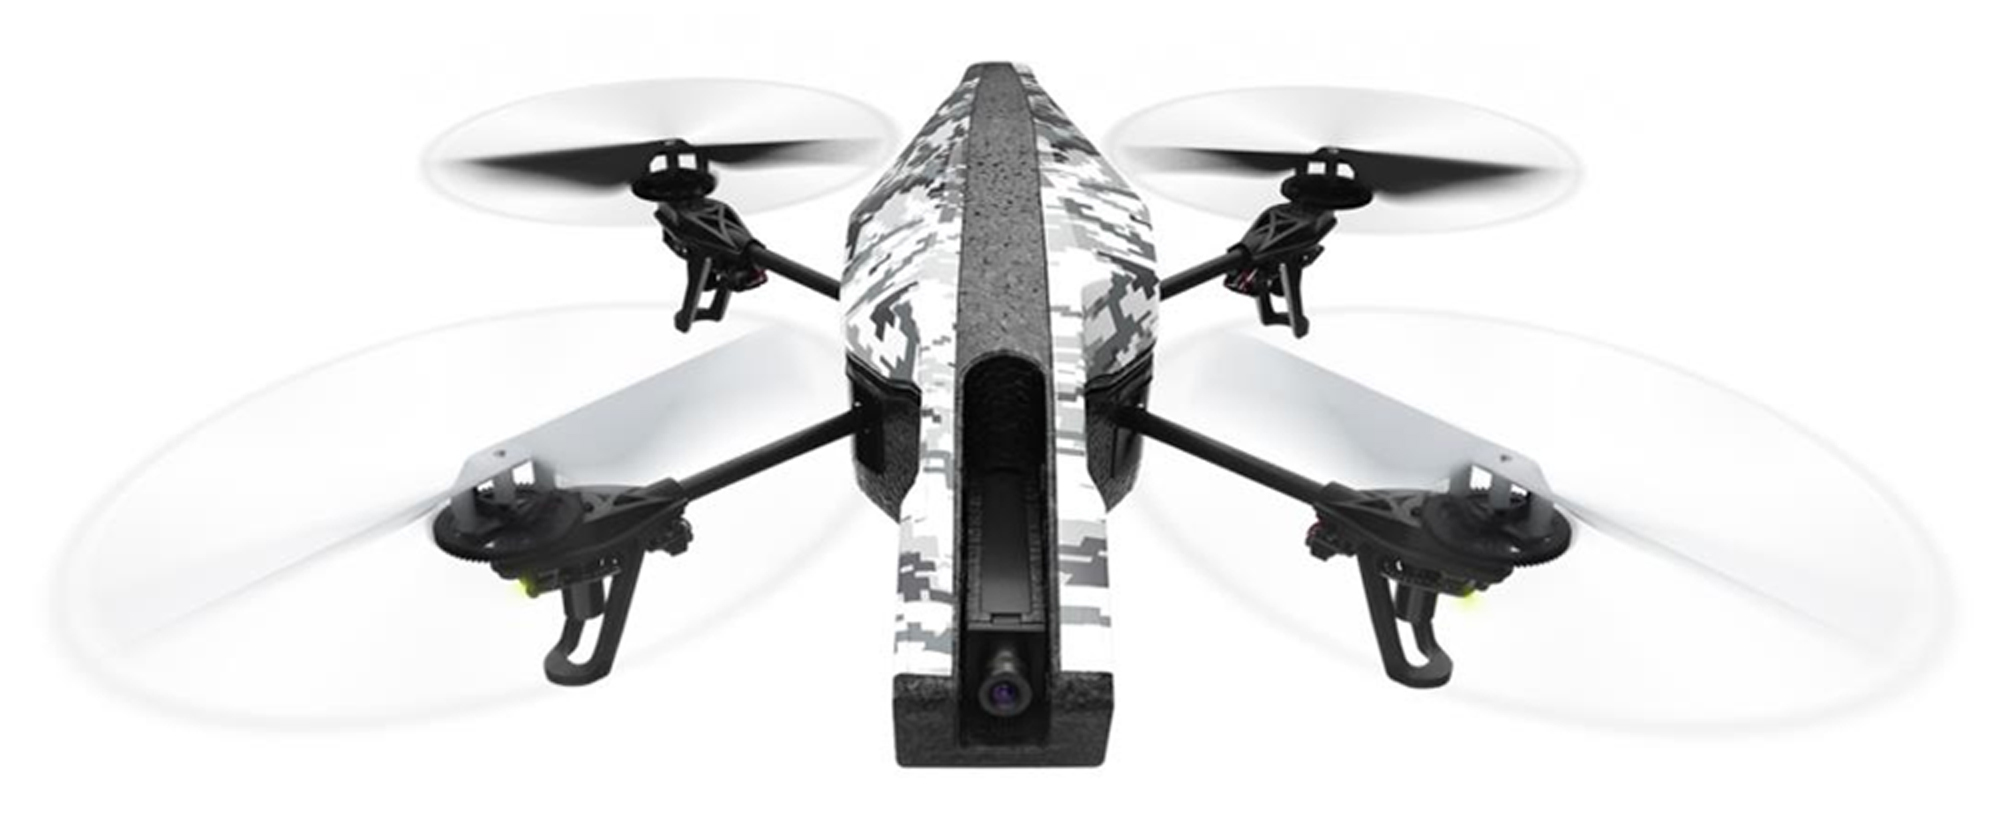
\includegraphics[width=0.7\textwidth]{images/ARDrone.jpg}
	\caption{Um \emph{AR.Drone}}
	\label{figARDrone}
\end{figure}
\end{frame}

\begin{frame}
\frametitle{Introdução}

A \emph{API} é boa, mas ainda um pouco baixo nível: 
\begin{itemize}
\item E.g.: Decolar, aplicar potência $p$ para frente
\item Seria útil poder fornecer um vetor posição $(\Delta x, \Delta y, \Delta z)$.
\end{itemize}

\vspace{2.5ex}

\textbf{Proposta:} Abstrair o movimento do AR.Drone. 

\end{frame}

\subsection{Metodologia}

\subsubsection{Procedimentos}

\begin{frame}
\frametitle{Metodologia}
Duas etapas principais do trabalho:
\begin{itemize}
\item Aprender a utilizar uma \emph{API} para controlar o drone.
\item Abstrair o controle de movimentos
\end{itemize}
\end{frame}

\subsubsection{API}

\begin{frame}
\frametitle{API}
Utilizamos o \emph{lib-ardrone}, uma biblioteca em \emph{python}
\begin{itemize}
\item Opensource
\item Abstração a nível de ação
\item Guiado para controle por teclado
\end{itemize}
\end{frame}

\subsubsection{Abstração do Controle}

\begin{frame}
\frametitle{Abstração do Controle}
\begin{itemize}
\item Controlador deve decompor um comando $(\Delta x, \Delta y, \Delta z)$ em ações únicas
\item Conversão de unidades de potência para $m/s$ e $rad/s$.
\item Regressão não-linear com dados experimentais.
\item Equações do tipo: 

\[
tempo(potencia) = \frac{a}{potencia^b} + c
\]

\end{itemize}
\end{frame}


\begin{frame}
%\frametitle{Abstração do Controle}
\begin{figure}
\begin{subfigure}[b]{0.4\textwidth}
	\centering
	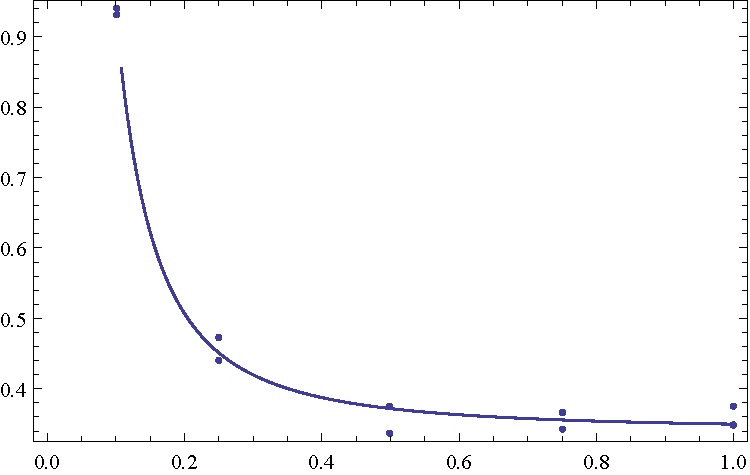
\includegraphics[width=\textwidth]{images/regressionForward.pdf}
	\caption{Para frente}
\end{subfigure}
\begin{subfigure}[b]{0.4\textwidth}
	\centering
	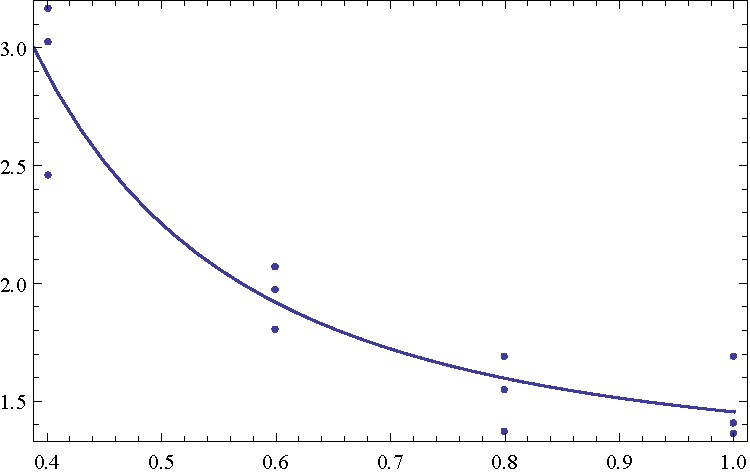
\includegraphics[width=\textwidth]{images/regressionUp.pdf}
	\caption{Para cima}
\end{subfigure}\\
\begin{subfigure}[b]{0.4\textwidth}
	\centering
	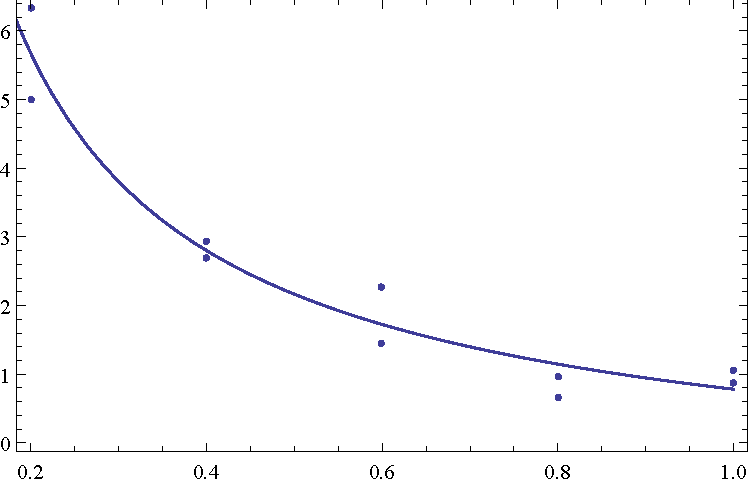
\includegraphics[width=\textwidth]{images/regressionDown.pdf}
	\caption{Para baixo}
\end{subfigure}
\begin{subfigure}[b]{0.4\textwidth}
	\centering
	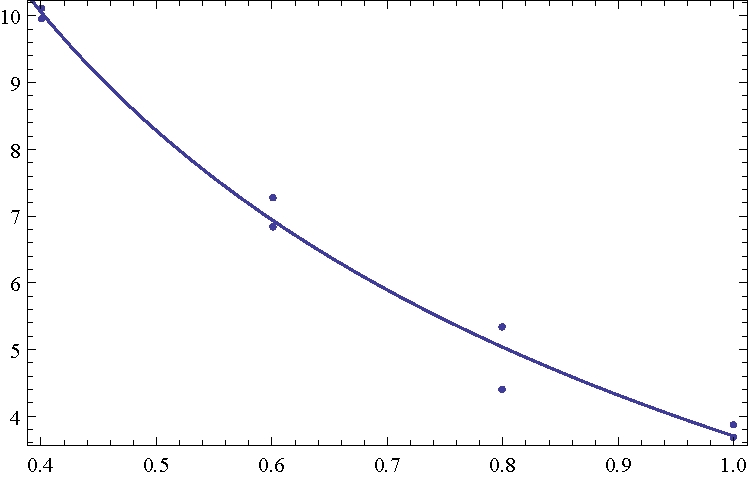
\includegraphics[width=\textwidth]{images/regressionAngular.pdf}
	\caption{Angular}
\end{subfigure}
\caption{Grafos $\text{tempo} \times \text{potência}$ dos resultados experimentais}
\end{figure}
\end{frame}

\subsection{Resultados}

\begin{frame}
\frametitle{Resultados}

Usando no controlador as inversas das funções experimentais, conseguimos fazer o \emph{AR.Drone} voar com (\emph{certa}) precisão
\vspace{3.0ex}
\begin{center}
\emph{[Vídeo: Robô comandado a voar até o meio da quadra (4.95m), girar uma vez ($2\pi$), subir (1m), descer(1m), e então pousar]}
\end{center}
\end{frame}

\section{Localização usando a câmera}

\subsection{Introdução}

\begin{frame}
\frametitle{Meta secundária: Localização usando a câmera}

A odometria no robô está sujeita a erro. É útil ter uma outra forma de se localizar
\vspace{2.0ex}

\textbf{Solução}: Usar a câmera de baixo para capturar imagens do chão, e comparar com um mapa.

\end{frame}

\subsection{Metodologia}

\begin{frame}
\frametitle{Meta secundária: Localização usando a câmera}
\begin{itemize}
\item Implementada usando a biblioteca \emph{opencv}
\item Testes usando o \emph{google mapas}, e imagens retiradas dele
\item Não houve tempo de integrar esta parte com o robô
\end{itemize}

\end{frame}

\subsection{Pseudocódigo}
\begin{frame}[fragile]

\begin{verbatim}
sift map = sift(map)
sift data = sift(data)
matches = knnmatch(sift map, sift data)
apply knn threshold(matches, 0.2)

theta = ∑(i, j = 0 to length(matches)) (angle from i to j in data - angle from i to j in map) / number of pairs
scale = ∑(i, j = 0 to length(matches)) (distance from i to j in data - distance from i to j in map) / number of pairs

for each i in matches:
        translate i relative to center of data
        rotate i in theta
        get the negative vector i so that it points from i to center of data
        apply scale to the vector
        apply the vector to the respective point in map
get the average of results
\end{verbatim}
\end{frame}

\begin{frame}
\begin{figure}
\begin{subfigure}[b]{0.4\textwidth}
	\centering
	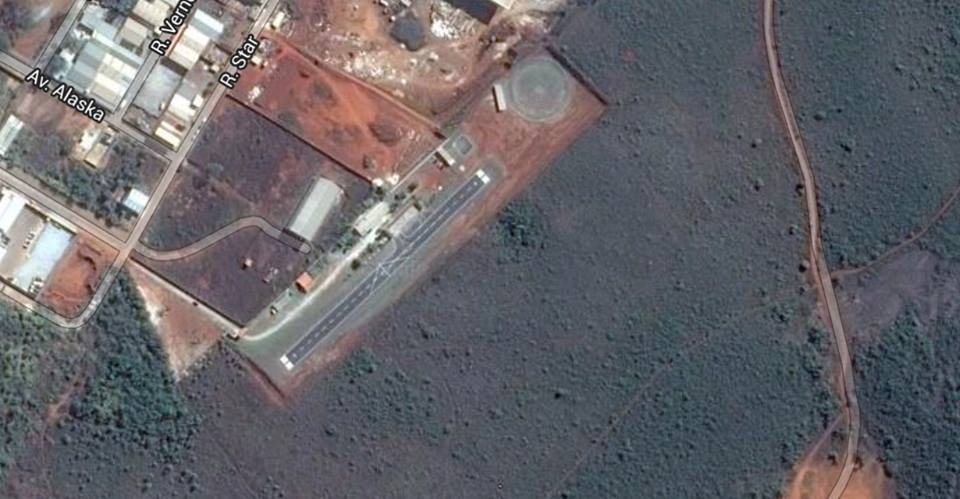
\includegraphics[width=\textwidth]{images/mapOriginal.png}
	\caption{Mapa original}
\end{subfigure}
\begin{subfigure}[b]{0.4\textwidth}
	\centering
	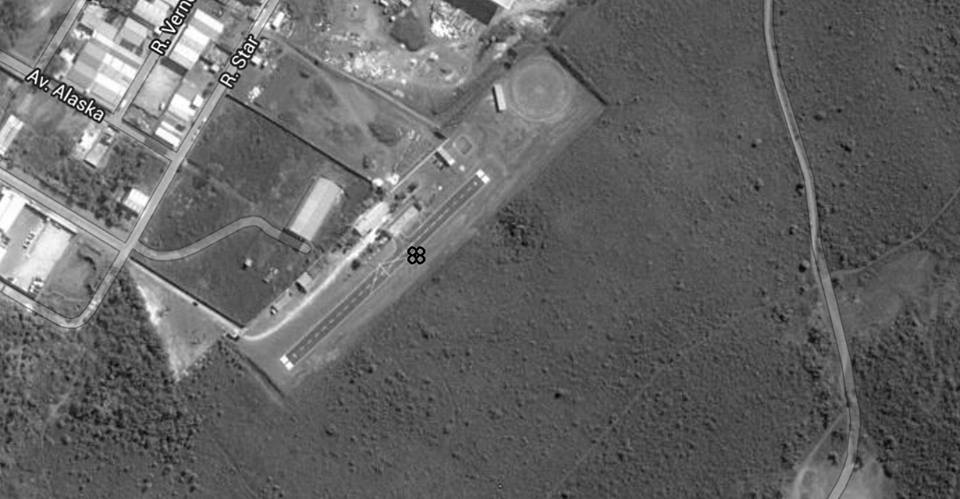
\includegraphics[width=\textwidth]{images/mapLocalized.png}
	\caption{Localização no Mapa}
\end{subfigure}
\caption{Objetivo e resultados do algoritmo}
\end{figure}
\end{frame}


\begin{frame}
\begin{figure}
\centering
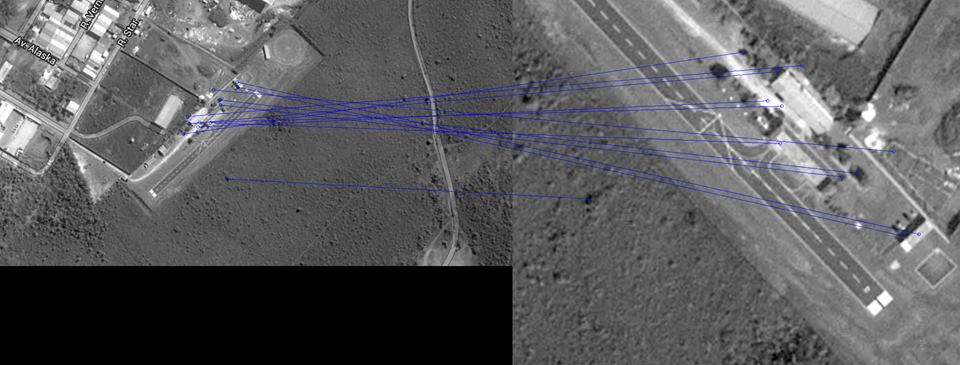
\includegraphics[width=\textwidth]{images/mapMatching.png}
\caption{Mapeamento do fragmento}
\end{figure}
\end{frame}

\section{Conclusão}
\begin{frame}
\frametitle{Conclusão}

Neste projeto, fizemos:
\begin{itemize}
\pause
\item Um controlador para o \emph{AR.Drone}, que abstrai seu controle para $(\Delta x, \Delta y, \Delta z)$
	\begin{itemize}
	\pause
	\item Usando o \emph{libardrone} como base
	\pause
	\item Efetuando medições experimentais para garantir a correspondência robô/mundo
	\end{itemize} 
\pause
\item Código de localização via imagens
	\begin{itemize}
	\pause
	\item Usando o \emph{opencv}
	\pause
	\item Testado no \emph{google mapas}
	\pause
	\item (dificuldades impediram seu uso no drone)
	\end{itemize}
\end{itemize}

\end{frame}

\begin{frame}
\begin{center}
\textbf{Obrigado!}
\end{center}
\end{frame}

\end{document}
